\pagebreak
\section{Example}\label{example}
This section shows an example model created using the plug-in. I describe
how to create it and how to analyze it.
\subsection{Project Creation}
You will first have to create a new empty project in Eclipse.

\centeredpic{example/new_project}{0.2}{Create a new project}{fig:new_project}

Then select one of the empty project templates and create
a new empty sirius project. Give it a name and create the
empty project. Then, right click on the new empty project
and go to \textbf{New}, then \textbf{Other}. 
\begin{figure}[H]
    \centering
    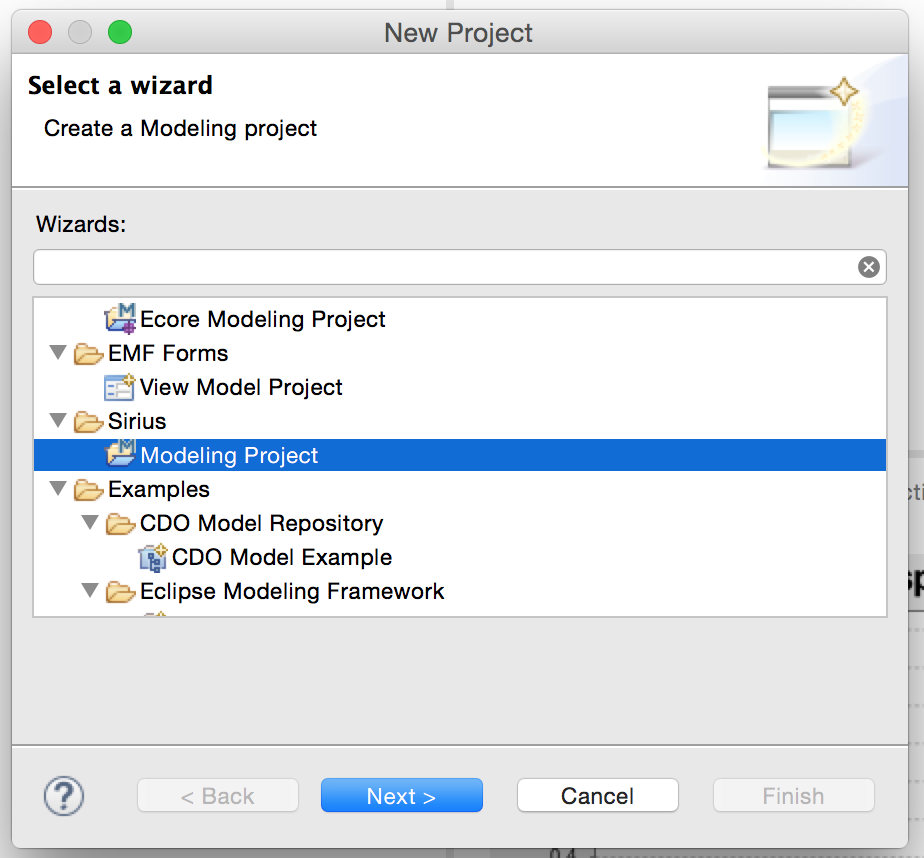
\includegraphics[width=0.3\textwidth]{example/select_project}
    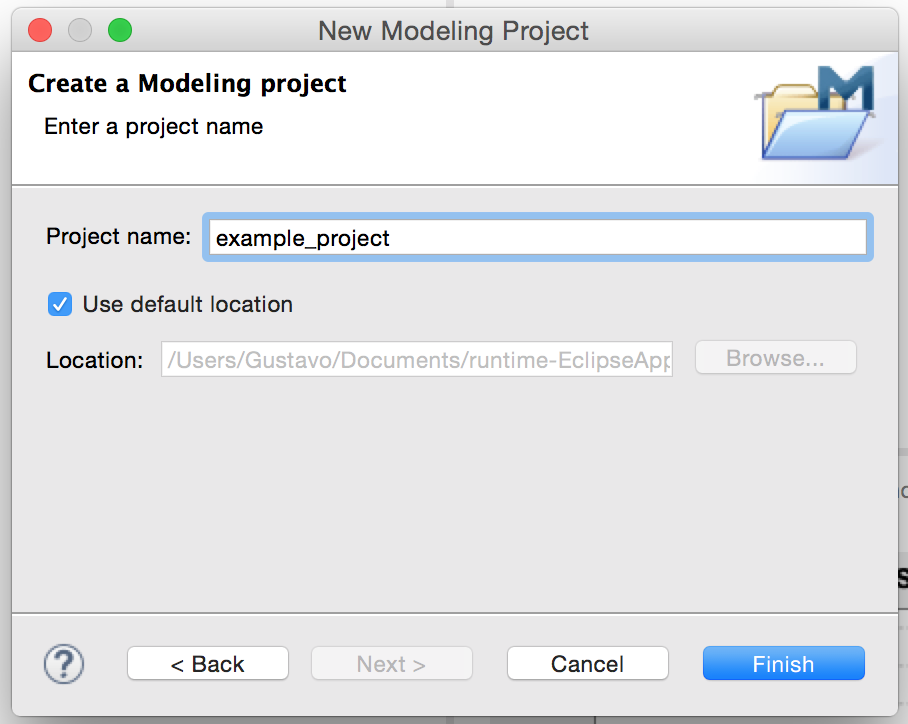
\includegraphics[width=0.3\textwidth]{example/name_project}
    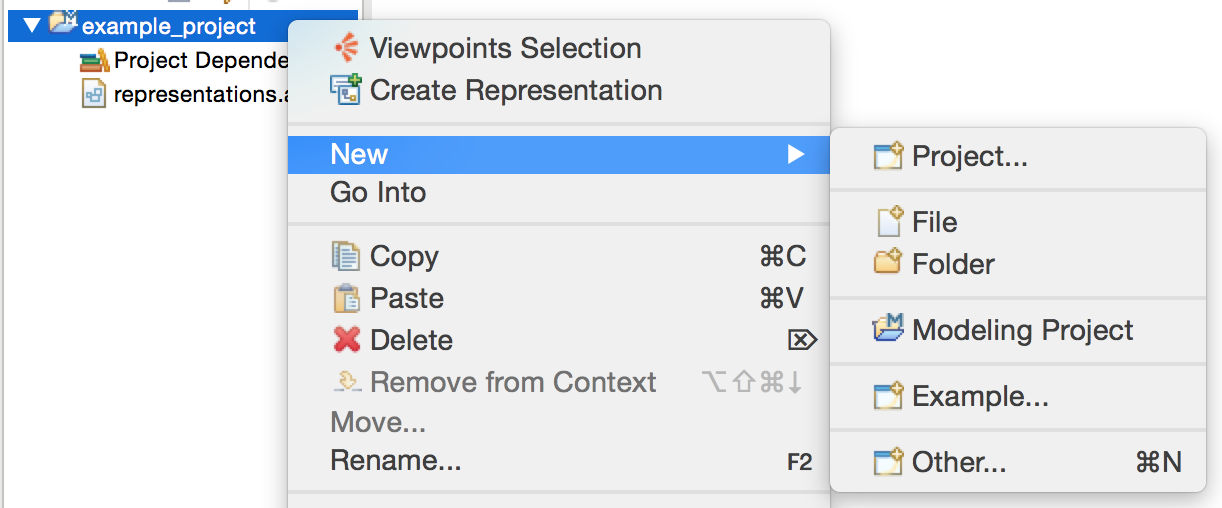
\includegraphics[width=0.3\textwidth]{example/new_model}
    \caption{Creation}
\end{figure}

Here you can search for the \texttt{Realtimescheduling model} to create
an instance of the model. Select the model and create it with a name.
When prompted, make sure to select the root element \texttt{System}.
\begin{figure}[H]
    \centering
    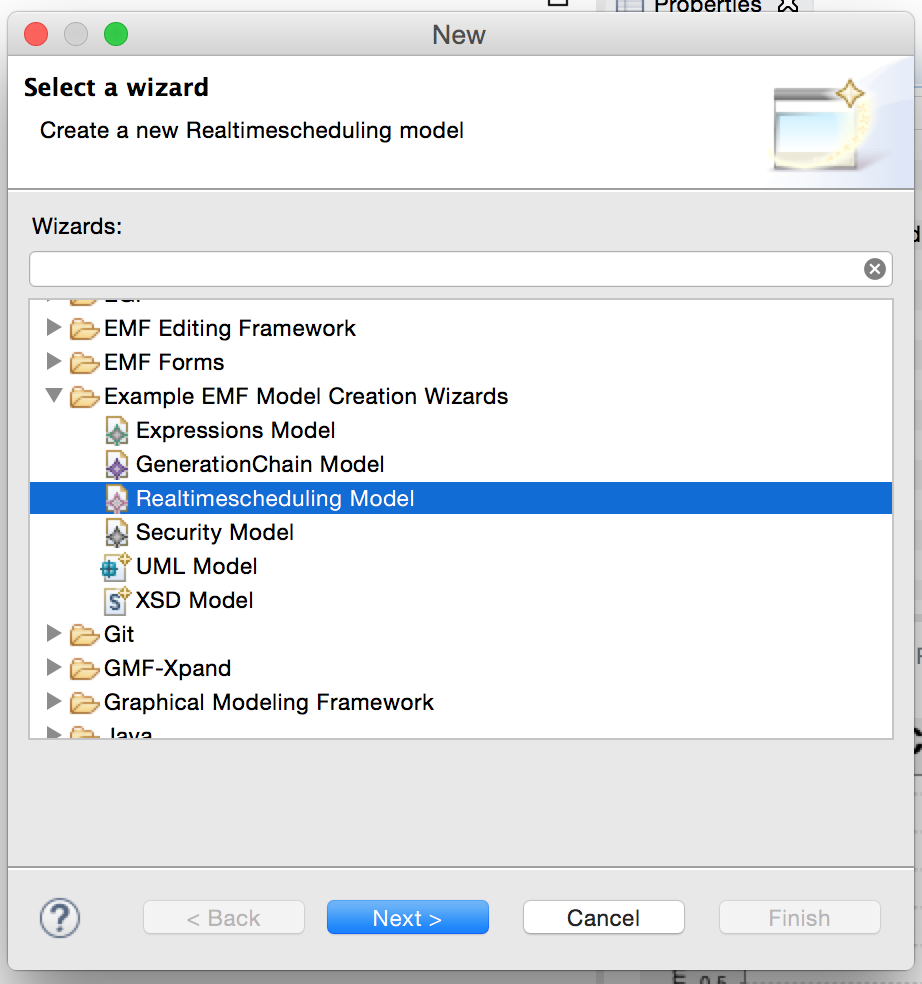
\includegraphics[width=0.4\textwidth]{example/select_model}
    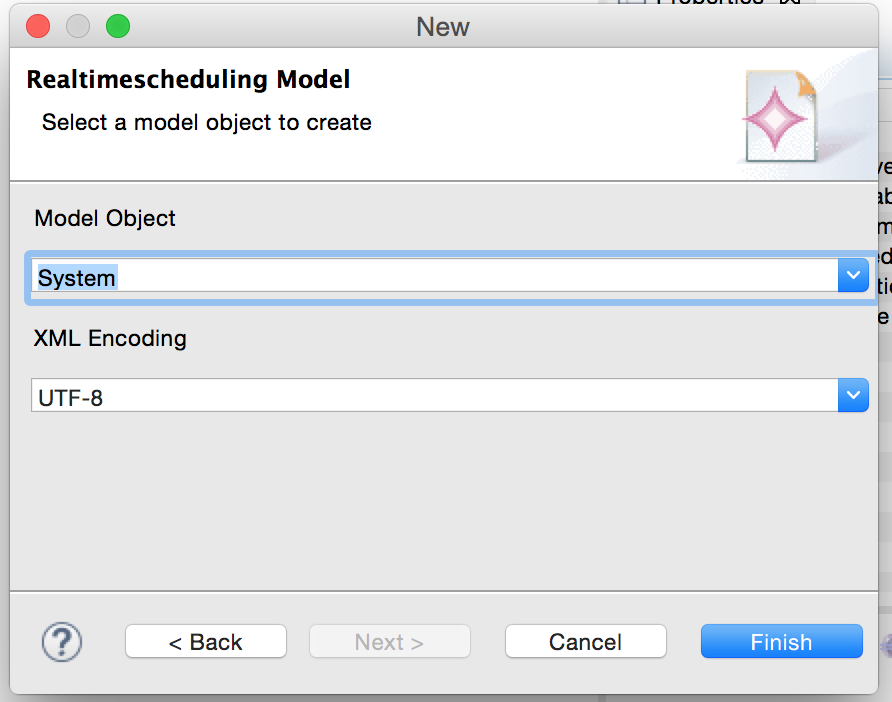
\includegraphics[width=0.4\textwidth]{example/root_element}
    \caption{Select model}
\end{figure}

\subsection{Manipulation}
You should change into the \texttt{Realtime Analysis} perspective to
maximize your use of the plugin. You should see the editor view appear
with a single element that is the \texttt{System} object. You will need
to define the model instance by compositional relations first. This
can be done by right-clicking on an element and adding children or sibling
objects.
\centeredpic{example/children}{0.3}{Adding children}{fig:children}

When you select a model element, the properties editor should change to display
the attributes of the element. Here you can change any attribute declared
as \texttt{changeable} by double clicking on the value field and
entering a new value.
\centeredpic{example/properties.png}{0.4}{Properties}{fig:properties}
Some of the fields will set referential relations and will ask
you to choose from a list of instance objects: for example, if you
were to set the Tasks of a partition then a window will open to display
all the tasks available. For this example, we will work on a ficticious quadcopter system where
the attitude controller tasks have hard realtime constraints.
Lets add some tasks and partition definitions. 
\centeredpic{example/defined_system.png}{0.2}{Defined system}{fig:system}
Now we can start probing the system but first we would like to make sure that
the system is ``Valid'' first: that it is structurally sound. We can
do that by right-clicking on the \texttt{System} object and 
then clicking on \texttt{Validate}.
\centeredpic{example/validate}{0.3}{Validate}{fig:validate}
If the model successfully validates, we should see an ``Success''
message. But if it does not, we will see errors on the objects
that did not pass validation.
\begin{figure}[H]
    \centering
    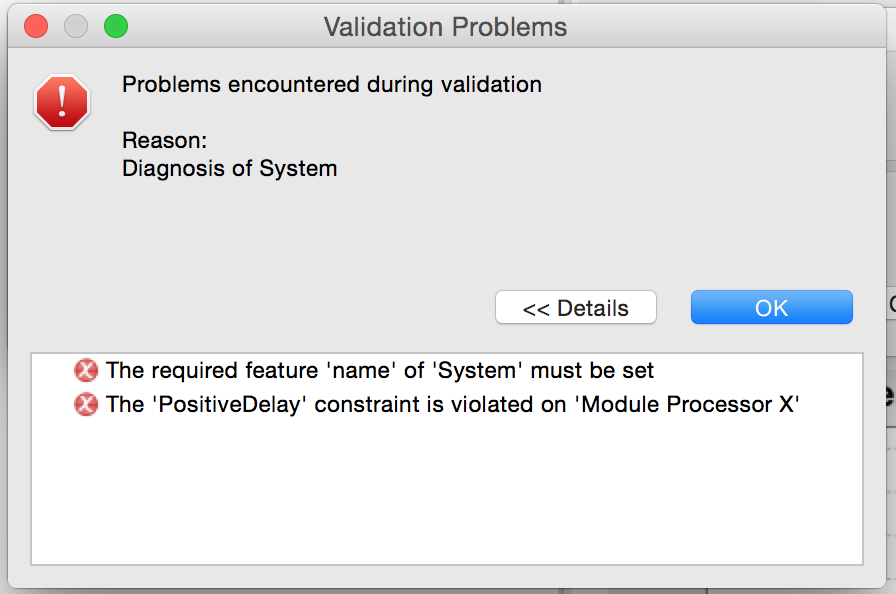
\includegraphics[width=0.4\textwidth]{example/validation_errors}
    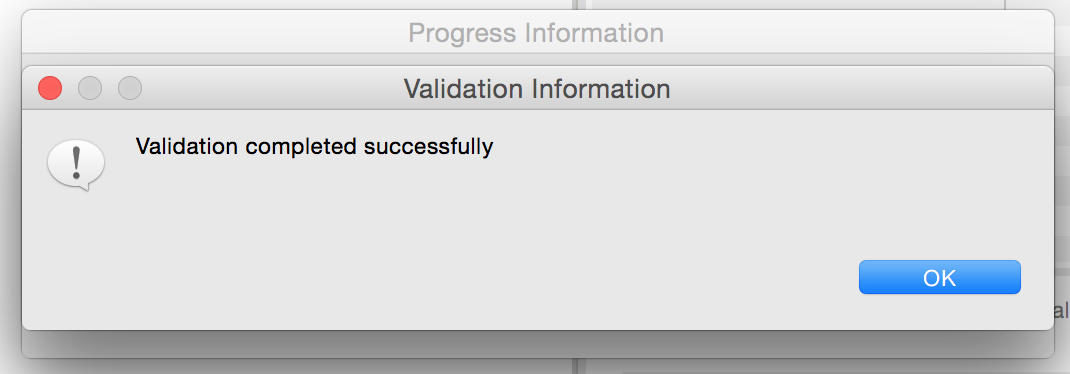
\includegraphics[width=0.4\textwidth]{example/validation_success}
    \caption{Validation messages}
\end{figure}
We can quickly fix the errors and see the expected success prompt.
Once the model has successfully validated, we can safely perform
analysis on it.
\subsection{Analysis}
Open the \textbf{Analysis} menu in the main
toolbar to see the possible options.
\centeredpic{example/analysis}{0.4}{Analysis menu}{fig:analysis}
We have not defined a network yet so we are constrained to analyzing
the tasks schedulability behavior.
Click on \textbf{Analysis} then \textbf{Response Time}.
This will run the analysis algorithm described in this paper
and display the results per-partition and per-task.
Here we can see that the \texttt{Motors} tasks will miss its deadline.
We can also take a look at the \textbf{Response Time} view to see
a bar chart of the worst case response time for all tasks in the system.
\begin{figure}[H]
    \centering
    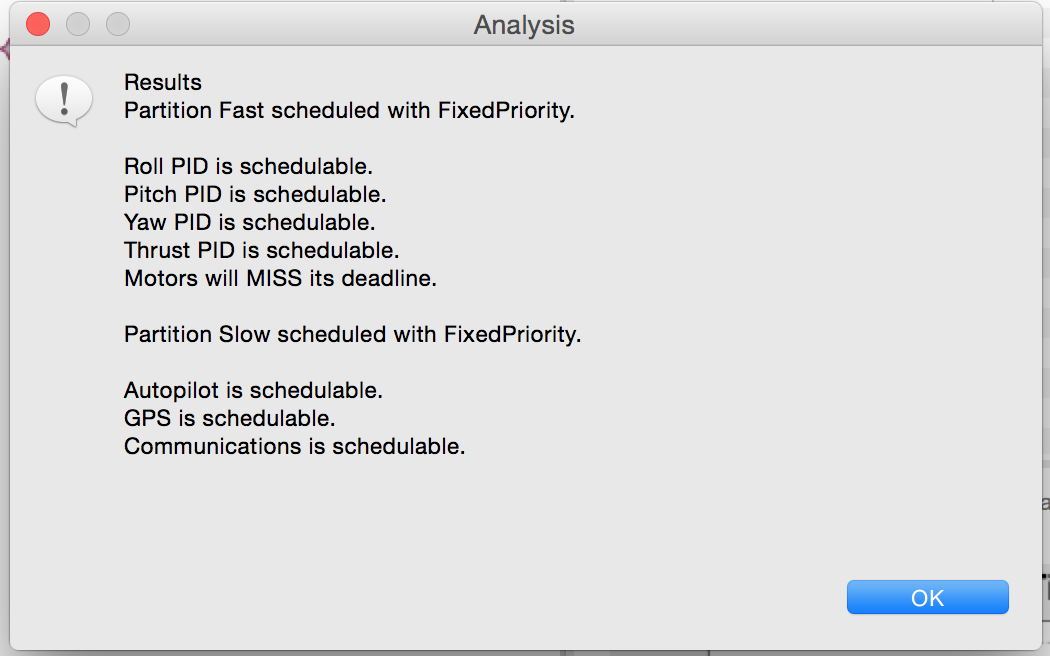
\includegraphics[width=0.4\textwidth]{example/analysis_results}
    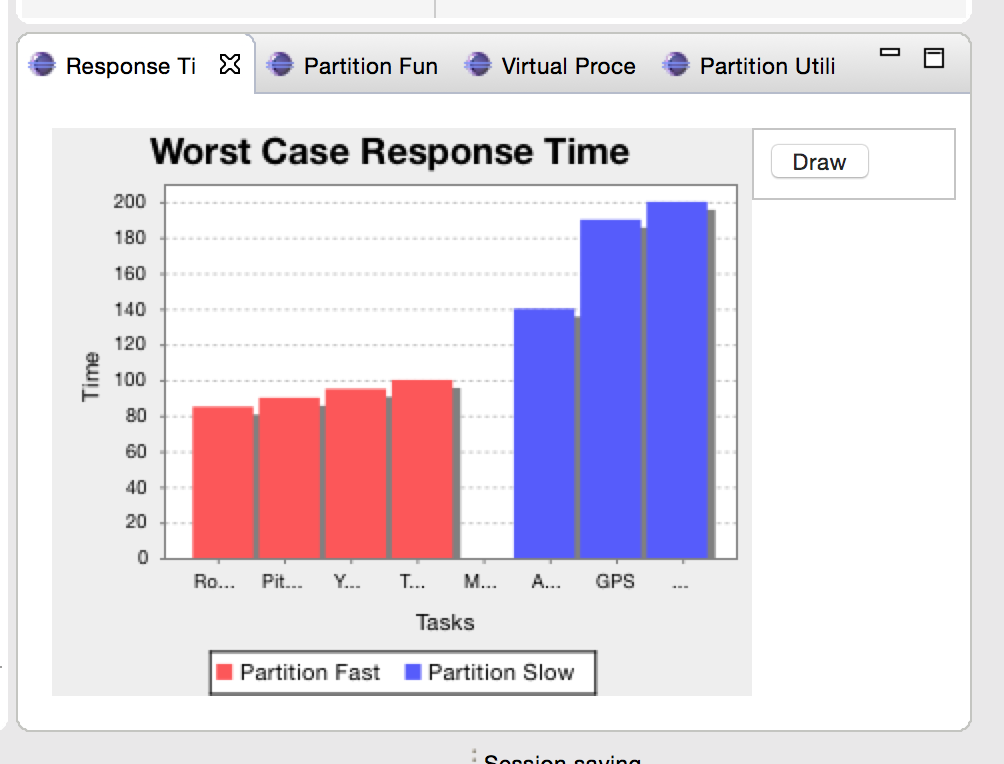
\includegraphics[width=0.5\textwidth]{example/graph_wcrt}
    \caption{Analysis results}
\end{figure}
We have a problem with the Motors missing their deadline. We have several
options as designers: we can decrease the execution time of the tasks,
we can increase its period, we can redistribute the time in the parititions,
or we can move it into a different partition.
The first and the last options are the most difficult: it might not be
possible to write faster code and it may be unsafe to move such a critical
task to a partition with lower priority tasks. The other two are tractable:
we will add more time to the ``Fast'' partition and increase the period
of the Motors task. Rerunning the analysis will show us that all tasks
are now schedulable.
\centeredpic{example/alter_partitions}{0.4}{Scheduling success}{fig:sched_success}
Now that a stable configuration is achieved, we can start thinking about 
adding new functions to the system. For example, we would like to add an
altitude control task to run alongside the PID controllers.
We define a new task with $T,D = 200$ and $C = 50$. Unfortunately this
tasks becomes unschedulable.
\centeredpic{example/new_task_misses}{0.4}{Scheduling failure}{fig:fail}
We can try to make it schedulable through trial and error but the plugin
can provide some information to help us make these decisions.
In the \texttt{Partition Functions} view, we can see that the \texttt{Least Supply}
function curve for the ``Fast'' partition has a value of 60 for $t = 200$. This
means that for all intervals of time of length 60, the minimum amount of supply
available is 60. This task requires 50 supply to complete but it must share
that with the other PID controller's tasks. Therefore by examining the least-supply
function and the other tasks in the system, we can estimate that this task
is unschedulable because for its period (200), there is barely enough time
to complete it and in fact the other tasks are canibalizing the time
for the altitude controller. If we want a safe cushion of time for this task,
we can look at larger values for the period in the least-supply curve.
We can also attempt to make this task a higher priority task manually
by assigning it a higher priority as a property. However, this 
has disastrous results. 
\centeredpic{example/bad_results}{0.4}{Priority changes do not fix the problem}{fig:a}
Notice that tasks in the ``Slow'' partition are unaffected by our changes to the
``Fast'' partition. This isolation is good for the designer but also for
the system where tasks will not harm the execution of other partition
if something goes wrong. We will force the system to be schedulable
by reducing the execution time of the Altitude controller but remember
that there are other means to do so.
We can look at the virtual processor utilization of a partition
to help us decide where to place new tasks. This function is in the
\textbf{Analysis} menu. 
\centeredpic{example/vpu_results}{0.4}{Virtual processor utilization}{fig:b}
The ``Fast'' partition has a relatively high VPU: around 75\%. The slow partition's
low VPU makes it a candidate for adding more tasks because the partition is only
being utilized for 20\% of the time it is executing. There is also a VPU view
chart available. Let's say that we want the drone to provide mobile wifi access.
We define some new tasks. 
\begin{figure}[H]
\centering
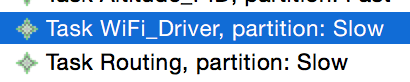
\includegraphics[width=0.4\textwidth]{example/new_slow_tasks}
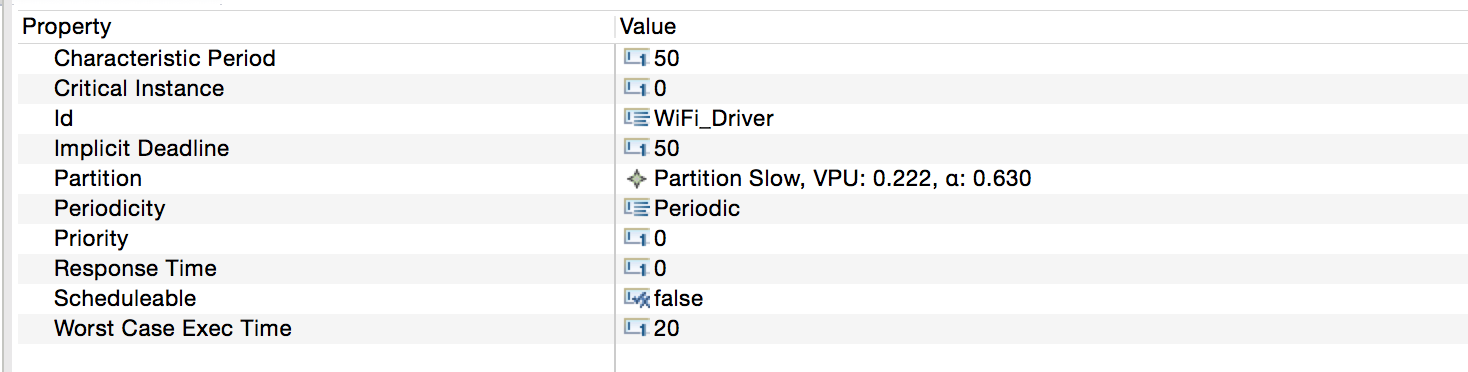
\includegraphics[width=0.4\textwidth]{example/new_slow_tasks_properties}
\caption{New wifi tasks}
\end{figure}
Immediately we see that these new tasks are unschedulable, but only in the 
``Slow'' partition! 
\centeredpic{example/missed_deadlines_within_partition}{0.5}{Local partition effects}{fig:z}
Let us look to the least supply function for guidance. 
The LSF for the ``Slow'' partition has a value of 0 at $t = 50$ which is
the period of the wifi tasks.
\centeredpic{example/least_supply_again}{0.5}{Least supply for ``Slow''}{fig:y}
This means that no task with a period less than $t = 130$ will ever complete in the slow
partition because there is a critical instance where the task will not get to execute for
130 time units. This lines up with the times $(0,130)$ which the ``Fast'' partition
claimed. Knowing this, we must make these tasks have longer periods. Once we make them
schedulable we can then see that this increases the VPU of the ``Slow'' partition.
\centeredpic{example/higher_vpu}{0.5}{Increased VPU}{fig:q}
\subsection{Network}
Now we will define a network component, although quadcopters do not communicate with motors
based on packet switched networks.
